\documentclass{article}
\usepackage{pgfplots}
\usetikzlibrary{pgfplots.groupplots}
\pgfplotsset{compat=1.7}


\begin{document}
	\thispagestyle{empty}

	\begin{figure}[t]
		\centering
		
		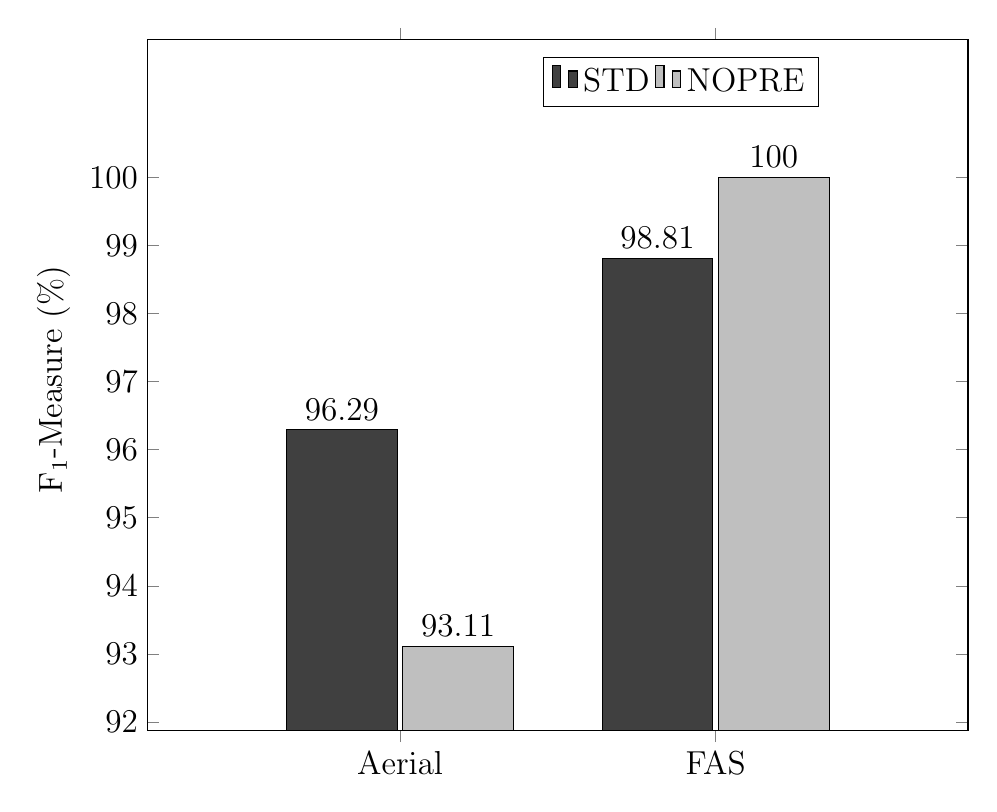
\begin{tikzpicture}
		\begin{axis}[
		width=12cm,
		ybar,
		enlargelimits=0.80,
		legend style={at={(0.65,0.975)},
		anchor=north,legend columns=-1},
		ylabel={\ F$_1$-Measure (\%)},
		symbolic x coords={Aerial,FAS},
		xtick=data,
		nodes near coords,
		nodes near coords align={vertical},
		bar width=40pt,
		style={font=\large},
		ytick={92,93,...,100},
		ymax=98.9,
		ymin=95
		]
%						STD		NPRE
%			Aerial
%				Clean	96.29	93.11
%				Noisy   97.22   96.92

%			FAS		
%				Clean	98.81	100
%				Noisy   99.62	99.62

			
		\addplot [color=black,fill=darkgray] coordinates {(Aerial,96.29) (FAS,98.81) };
		\addplot [color=black,fill=lightgray] coordinates {(Aerial,93.11) (FAS,100) };
		
%		\addplot [color=black,fill=darkgray] coordinates {(Aerial,97.22) (FAS,96.92) };
%		\addplot [color=black,fill=lightgray] coordinates {(Aerial,99.62) (FAS,99.62) };
		
		\legend{STD,NOPRE}
		\end{axis}
		\end{tikzpicture}
		%\vspace{-0.7cm}
		%\caption{Left: the pitch distribution for the 10 male speakers. Right: the active speech level for the 20 speakers.}\label{fig:pitch}
		%\vspace{-0.5cm}
	\end{figure}


\end{document}